
\begin{figure}[ht!]
	\centering
	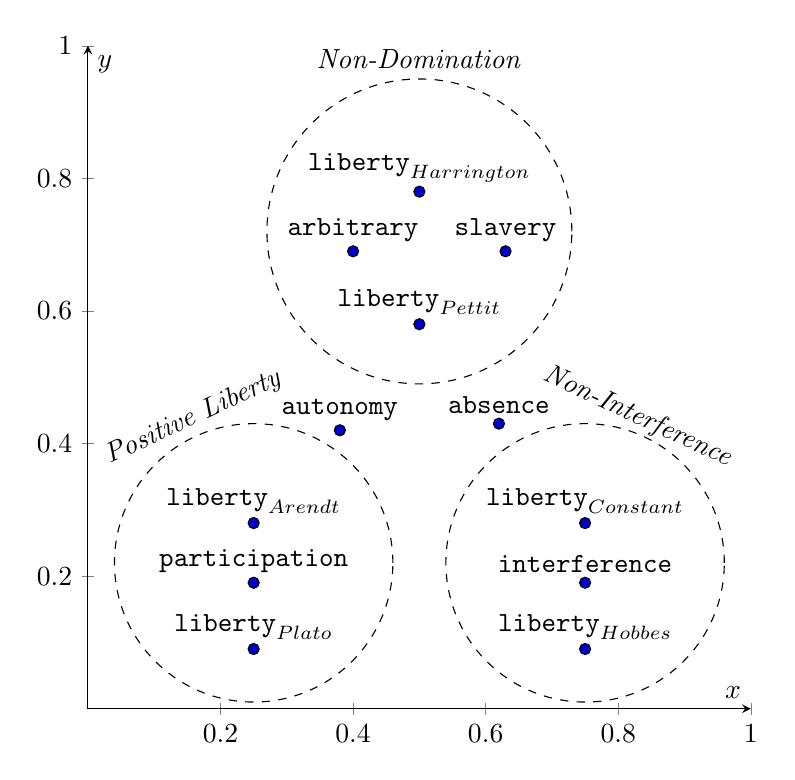
\begin{tikzpicture}
		\begin{axis}[axis lines=center,
			%view={28}{22},
			xmin=0, xmax=1, ymin=0, ymax=1,
			%xtick={0,1},ytick={0,1.0},
			xlabel=$x$,ylabel=$y$,width=10cm,height=10cm]
			\addplot+[only marks,point meta=explicit symbolic, nodes near coords,black] coordinates 
			{
				% top left: withdrawal_drugs
				(0.5,0.78)[$\texttt{liberty}_\text{Harrington}$]
				(0.5,0.58)[$\texttt{liberty}_\text{Pettit}$]
				(0.4,0.69)[$\texttt{arbitrary}$]
				(0.63,0.69)[$\texttt{slavery}$]
				% bottom left: bank_money
				(0.25,0.28)[$\texttt{liberty}_\text{Arendt}$]
				(0.25,0.09)[$\texttt{liberty}_\text{Plato}$]
				(0.25,0.19)[$\texttt{participation}$]
				(0.38,0.42)[$\texttt{autonomy}$]
				% top right: bank_water
				% waves
				%(0.8,0.8)[{\includesvg[width=5.5mm]{./ch0/figs/1F30A.svg}}]
				% droplet
				(0.62,0.43)[$\texttt{absence}$]
				(0.75,0.28)[$\texttt{liberty}_\text{Constant}$]
				(0.75,0.09)[$\texttt{liberty}_\text{Hobbes}$]
				(0.75,0.19)[$\texttt{interference}$]
				% bottom right: stream_music
				% 3 notes
				%(0.8,0.19)[{\includesvg[width=5.5mm,height=5.5mm]{./ch0/figs/1F3B6.svg}}]
				% 1 note
				%(0.8,0.3)[$\textsf{stream}_2$]
			};
			%\addplot+ graphics[xmin=0,xmax=96,ymin=0,ymax=96] {Dad64.png};
			% Positive Liberty + Circle
			\node[rotate=25] (a) at (axis cs:0.16,0.44) {\textit{Positive Liberty}};
			\draw[dashed] (axis cs:0.25,0.22) circle [blue, radius=0.21];
			\node[rotate=-25] (a) at (axis cs:0.83,0.44) {\textit{Non-Interference}};
			\draw[dashed] (axis cs:0.75,0.22) circle [blue, radius=0.21];
			% Non-Domination + Circle
			\node[] (a) at (axis cs:0.5,0.98) {\textit{Non-Domination}};
			\draw[dashed] (axis cs:0.5,0.72) circle [blue, radius=0.23];
		\end{axis}
	\end{tikzpicture}
	\caption{A visualization of \BERT{}'s ability to model the different contexts (and thus, senses) in which words are used by different authors. In this case \texttt{interference} falls squarely within the negative liberty (liberty as non-interference) cluster, as a term central to distinguishing negative from other forms of liberty, whereas \texttt{absence} falls between two clusters as it can be employed in both republican (``absence of arbitrary power'') and negative-liberty (``absence of interference'') contexts.}
	\label{fig:bert-author}
\end{figure}
